\documentclass[11pt,a4paper]{article}
\usepackage[utf8]{inputenc}
\usepackage[T1]{fontenc}
\usepackage{babel}
\babelprovide[import,main,hyphenrules=nohyphenation]{italian}
\usepackage{mathptmx}
\usepackage[scaled=0.92]{helvet}
\usepackage{courier}
\usepackage{microtype}
\usepackage[margin=2.4cm]{geometry}
\usepackage{amsmath,amssymb}
\usepackage{booktabs}
\usepackage{array}
\usepackage{xcolor}
\usepackage{listings}
\usepackage{tikz}
\usetikzlibrary{arrows.meta,positioning,fit,calc}
\usepackage{pgfplots}
\pgfplotsset{compat=1.18}
\usepackage{caption}
\usepackage[hidelinks]{hyperref}
\usepackage{enumitem}
\setlist{itemsep=2pt,topsep=4pt}
\setlength{\emergencystretch}{3em}

\definecolor{kw}{RGB}{0,70,140}
\definecolor{cm}{RGB}{110,110,110}
\lstdefinelanguage{Kairos}{
  morekeywords={procedure,int,stack,channel,local,delocal,call,uncall,if,then,else,fi,
    from,do,loop,until,par,and,rap,push,pop,show,skip,nil,empty,ssend,srecv},
  sensitive=true, morecomment=[l]{//}}
\lstset{language=Kairos, basicstyle=\ttfamily\small, keywordstyle=\color{kw}\bfseries,
  commentstyle=\color{cm}\itshape, columns=fullflexible, keepspaces=true,
  frame=single, framerule=0.3pt, rulecolor=\color{black!25}, xleftmargin=4pt,
  xrightmargin=4pt, aboveskip=6pt, belowskip=6pt, showstringspaces=false}
\newcommand{\kw}[1]{\texttt{#1}}

\title{\textbf{kgzip2: un compressore reversibile in Kairos}\\[4pt]
\large Il decompressore come inverso del compressore, e l'ordinamento delle rotazioni in $O(n\log n)$}
\author{Nicolò Giuliani\\[2pt]\small Università di Bologna, relazione tecnica, ottobre 2026}
\date{}

\begin{document}
\maketitle

\begin{abstract}
In un linguaggio reversibile comprimere e decomprimere non sono due programmi da tenere allineati: il decompressore è il compressore eseguito all'indietro. Questo lavoro estende il caso di studio del capitolo 4 della tesi (trasformata di Burrows e Wheeler reversibile, a blocchi paralleli, dopo Lyngby et al.~\cite{lyngby}) a un compressore completo, \emph{kgzip2}, costruito sulla pipeline di bzip2: RLE iniziale, BWT, move-to-front, RLE degli zeri e codice di Elias gamma. Tutto è una sola procedura Kairos, \kw{comprimi}. Il programma di decompressione riceve soltanto i bit compressi e cinque contatori per blocco ed esegue \kw{uncall comprimi(...)}: nel sorgente non esiste una riga di decodifica. Perché questo funzioni ogni stadio è \emph{pulito}: consuma l'ingresso e lascia solo l'uscita, compresa la BWT, che nel capitolo 4 lasciava il blocco originale. Il secondo contributo riguarda il punto che~\cite{lyngby} indica come miglioramento necessario, l'ordinamento delle rotazioni: dal bubble sort $O(n^3)$ si passa a un confronto con uscita anticipata, a un merge sort reversibile e infine a un ordinamento per raddoppio dei prefissi, $O(n\log n)$ qualunque siano i dati. @@ABSTRACT_NUMERI@@ L'eseguibile \kw{kgzip2} è un file unico che funziona senza Kairos installato e lavora in streaming, a gruppi di blocchi: la memoria resta costante qualunque sia la dimensione del file. Infine, un file alterato che sfugga al CRC quasi sempre ferma la VM da sola: le condizioni che rendono il programma invertibile, lette all'indietro, diventano controlli dell'ingresso che nessuno ha scritto.
\end{abstract}

\section{Introduzione}

La compressione lossless è il banco di prova naturale per un linguaggio reversibile. Comprimere e decomprimere sono l'una l'inversa dell'altra, quindi in un linguaggio in cui ogni programma ha un inverso calcolabile basta scriverne una metà, e le due metà non possono divergere. Il prezzo è che ogni passo deve conservare l'informazione: niente cancellazioni, niente variabili sovrascritte, niente uscite anticipate da un \kw{if}.

Lyngby, Nylandsted, Glück e Yokoyama~\cite{lyngby} hanno scritto in Janus versioni reversibili e \emph{pulite} di due algoritmi dello standard zip, LZW e la BWT. La loro BWT ordina le rotazioni con un algoritmo ingenuo, $O(n^3)$, e il lavoro conclude che migliorare quell'ordinamento è possibile e necessario. Il loro lavoro è sequenziale. Il capitolo 4 della tesi ha portato la BWT in Kairos e ha trasformato i blocchi in parallelo, come rami di un \kw{par}.

Questo lavoro fa il passo successivo: un compressore intero, da file a file, con la decompressione ottenuta per inversione. I contributi:
\begin{enumerate}
\item \textbf{kgzip2}, una pipeline nello stile di bzip2~\cite{bzip2} (RLE, BWT, MTF, RLE degli zeri, codice a prefisso) scritta come un'unica procedura pulita; la decompressione è \kw{uncall} della stessa procedura;
\item la \textbf{BWT pulita in senso stretto}: anche l'ingresso viene azzerato, che era uno dei limiti dichiarati del capitolo 4;
\item una sequenza di \textbf{ordinamenti reversibili delle rotazioni} che porta il costo da $O(n^3)$ a $O(n\log n)$ indipendentemente dai dati, con le tecniche che servono a renderli reversibili;
\item una \textbf{valutazione}: correttezza byte per byte, rapporto di compressione contro bzip2, tempi, casi peggiori, concorrenza.
\end{enumerate}

\section{Contesto}

\paragraph{Kairos.} Linguaggio reversibile e concorrente della famiglia di Janus~\cite{janus}: assegnamenti reversibili (\kw{+=}, \kw{-=}, \kw{<=>}), condizionali con asserzione d'uscita (\kw{if} $e_1$ \kw{then} \dots\ \kw{fi} $e_2$), cicli \kw{from} $e_1$ \kw{do} \dots\ \kw{until} $e_2$, blocchi \kw{local}/\kw{delocal}, \kw{call}/\kw{uncall}, array, stack, \kw{par} e canali sincroni. Le guardie sono espressioni con \kw{\&\&} e \kw{||}; gli stack hanno \kw{push} e \kw{pop} ma non un'operazione per leggere la cima. Il frontend è in Python e produce bytecode testuale; la macchina virtuale, in C, lo esegue nei due versi.

\paragraph{Pulito.} Un algoritmo reversibile non può cancellare. Lyngby et al. chiamano \emph{clean} un programma che lascia solo l'uscita. La tecnica è una coppia di procedure: una produce l'uscita e dei dati ausiliari, l'altra ricalcola gli stessi ausiliari partendo dall'uscita; chiamare la prima e disfare la seconda lascia la sola uscita. Per un compressore la pulizia è la condizione perché l'inverso sia un decompressore: se \kw{comprimi} lasciasse spazzatura, il suo inverso avrebbe bisogno anche di quella, che un file compresso non contiene.

\paragraph{Spazzatura alla Bennett.} Quando un passo non si può disfare subito, il dato che servirebbe a disfarlo va su uno stack (\kw{scarto}) e sparisce disfacendo l'intera procedura che l'ha prodotto~\cite{bennett}. È lo schema \kw{call ordina; call estrai; uncall ordina}: l'ordinamento lascia spazzatura, l'estrazione usa l'ordine, e l'ordinamento disfatto la porta via.

\paragraph{Testimoni.} Ogni \kw{if} deve dire in uscita quale ramo ha preso. Quando la condizione d'ingresso non è più verificabile dopo il corpo, si usa un testimone: una variabile che vale 1 solo se si è entrati, e che poi va azzerata deducendola dallo stato.

\section{\texttt{kgzip2 file.txt}, passo per passo}
\label{sec:pipeline}

Questa sezione descrive l'intero percorso come lo vede chi usa il programma. L'eseguibile esiste: \kw{dist/bin/kgzip2} è un file unico di circa 8 MB, costruito con PyInstaller, che funziona su una macchina senza Kairos né Python. Ha le opzioni di gzip e bzip2: \kw{-d}, \kw{-t}, \kw{-k}, \kw{-c}, \kw{-f}, \kw{-v}, \kw{-1}\dots\kw{-9}, più \kw{-T} per il numero di blocchi per esecuzione della VM, e senza file fa da filtro fra stdin e stdout. Lavora in streaming: un file di qualunque dimensione passa a gruppi di blocchi, con la memoria costante.

\subsection{Che cosa c'è dentro l'eseguibile}

\begin{itemize}
\item \textbf{la libreria Kairos} \kw{kgzip2.kairos}: tutti gli stadi e la procedura \kw{comprimi};
\item \textbf{il frontend Kairos} (lexer, parser LALR, controlli statici, generatore di bytecode), che traduce la libreria e un \kw{main} senza dati: poche centinaia di righe, in meno di un decimo di secondo;
\item \textbf{la macchina virtuale} (\kw{libvm.so}), che esegue il bytecode in avanti o all'indietro e realizza \kw{par} con un thread per ramo;
\item \textbf{un involucro} che legge e scrive i file in streaming, scrive i dati direttamente come istruzioni di bytecode e gestisce il formato a frame \kw{.kgz}. Non comprime nulla: sposta byte e impacchetta bit.
\end{itemize}

\noindent La VM gira in un processo figlio con un tempo massimo, così un programma che non terminasse non bloccherebbe il comando. La stessa costruzione produce \kw{klzma}.

\begin{figure}[t]
\centering
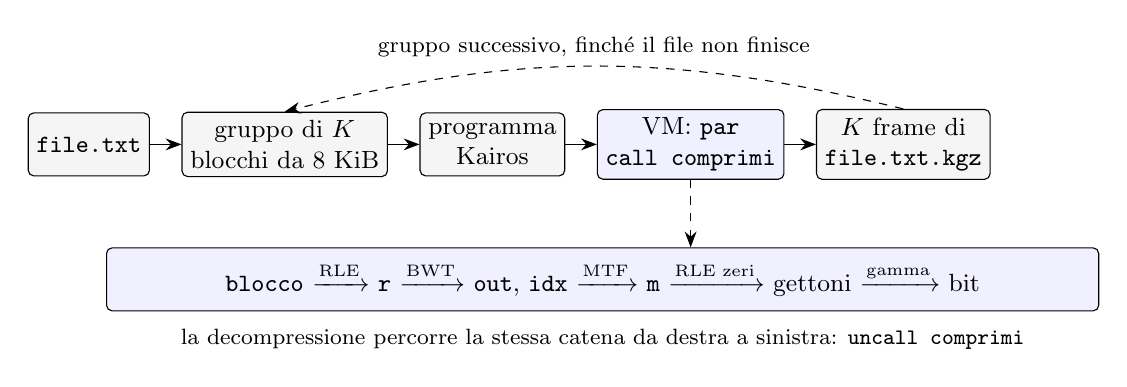
\begin{tikzpicture}[
  box/.style={draw, rounded corners=2pt, minimum height=8mm, align=center, font=\small, inner sep=3pt},
  kai/.style={box, fill=blue!6},
  py/.style={box, fill=black!4},
  >={Stealth[length=2mm]}, node distance=4mm and 4mm]
\node[py] (in) {\kw{file.txt}};
\node[py, right=of in] (bl) {gruppo di $K$\\blocchi da 8 KiB};
\node[py, right=of bl] (src) {programma\\Kairos};
\node[kai, right=of src] (vm) {VM: \kw{par}\\\kw{call comprimi}};
\node[py, right=of vm] (out) {$K$ frame di\\\kw{file.txt.kgz}};
\draw[->] (in) -- (bl); \draw[->] (bl) -- (src); \draw[->] (src) -- (vm); \draw[->] (vm) -- (out);
\draw[->, dashed] (out.north) to[bend right=14] node[above, font=\footnotesize] {gruppo successivo, finché il file non finisce} (bl.north);
\node[kai, below=9mm of src, minimum width=12.6cm, xshift=1.4cm] (stadi) {
\kw{blocco} $\xrightarrow{\text{RLE}}$ \kw{r} $\xrightarrow{\text{BWT}}$ \kw{out}, \kw{idx}
$\xrightarrow{\text{MTF}}$ \kw{m} $\xrightarrow{\text{RLE zeri}}$ gettoni $\xrightarrow{\text{gamma}}$ bit};
\draw[->, dashed] (vm.south) -- (vm.south |- stadi.north);
\node[font=\footnotesize, align=center, below=1mm of stadi] {la decompressione percorre la stessa catena da destra a sinistra: \kw{uncall comprimi}};
\end{tikzpicture}
\caption{Il percorso di \kw{kgzip2}. In grigio l'involucro, in azzurro ciò che esegue Kairos. Il ciclo si ripete per ogni gruppo di $K$ blocchi (uno per core): in memoria c'è un gruppo alla volta.}
\label{fig:pipeline}
\end{figure}

\subsection{Compressione}

\paragraph{1. Lettura a gruppi.} Il file si legge come flusso, a blocchi di $B$ byte ($B = 1024\cdot$livello, 8192 con \kw{-8}); l'ultimo può essere più corto. I blocchi sono indipendenti e si raccolgono in gruppi di $K$, uno per core (\kw{-T} lo cambia): ogni gruppo è un'esecuzione della VM, con i blocchi come rami di un \kw{par}, e i passi 2--4 si ripetono per ogni gruppo. In memoria ci sono solo i blocchi del gruppo corrente, più uno letto in anticipo per sapere qual è l'ultimo: la RAM non dipende dalla dimensione del file (§\ref{sec:memoria}), e il comando funziona anche da una pipe, senza conoscere la lunghezza dei dati. Un blocco di meno di 2 byte, che può essere solo l'ultimo, si memorizza senza passare dalla VM.

\paragraph{2. Caricamento.} La VM non legge file, quindi i dati entrano nello store del programma. L'involucro genera un \kw{main} che dichiara, per ogni blocco $i$, gli array di lavoro (tutti a zero) e contiene un segnaposto al posto dei dati. Solo questa parte passa dal frontend; al posto del segnaposto, nel bytecode, l'involucro scrive un'istruzione per byte, \kw{PUSHEQ blocco\_0[k] v}, cioè ciò che il frontend produrrebbe da \kw{blocco\_0[k] += v}:
\begin{lstlisting}
local int blocco_0[12] = 0
...
blocco_0[0] += 98      // 'b'
blocco_0[1] += 97      // 'a'
...
par
    call comprimi(blocco_0, r_0, ..., bit_0, idx_0, n1_0, ..., nr_0)
and
    call comprimi(blocco_1, r_1, ..., bit_1, idx_1, n1_1, ..., nr_1)
rap
show(idx_0)  show(n1_0)  show(ng_0)  show(nel_0)  show(nb_0)  show(bit_0)
\end{lstlisting}
Il parser non vede mai i dati: in decompressione, dove i bit sono decine di migliaia, questo toglie circa 5 secondi su 8 KiB. E poiché i gruppi pieni hanno tutti la stessa forma ($K$ blocchi da $B$ byte), il frontend traduce il programma una volta sola: ogni gruppo riusa lo stesso bytecode, con i propri dati al posto del segnaposto. Il trattino basso fra nome e indice non è estetico: senza, il contatore \kw{n1} del blocco 0 e la lunghezza \kw{n} del blocco 10 si chiamerebbero entrambi \kw{n10}, e da 11 blocchi in su il controllo statico di Kairos fermerebbe il programma per una corsa critica nel \kw{par} (è successo alla prima versione, che con blocchi da 8 KiB non comprimeva file oltre 80 KiB).

\paragraph{3. Esecuzione.} La VM esegue \kw{call comprimi} su ogni ramo in parallelo. I rami scrivono array disgiunti, quindi il controllo statico sul \kw{par} li accetta. Dentro \kw{comprimi} gli stadi si susseguono; ciascuno ha come precondizione l'uscita a zero e come postcondizione l'ingresso a zero. La Tabella~\ref{tab:esempio} segue un blocco di 12 byte.

\begin{table}[t]
\centering\small
\begin{tabular}{@{}l>{\raggedright\arraybackslash}p{10.6cm}@{}}
\toprule
stadio & stato dopo lo stadio \\
\midrule
ingresso & \kw{barbaaaaara!} = 98 97 114 98 97 97 97 97 97 114 97 33 \quad ($n=12$)\\
RLE iniziale & 98 97 114 98 \textbf{1 0 97 97 97 97} 114 97 33 \quad ($n_1 = 13$: la corsa di cinque \kw{a} diventa $(5-4) \bmod 256$, $(5-4) \operatorname{div} 256$, quattro copie)\\
BWT, ordine & \kw{offs} = 5 4 12 11 6 7 8 9 1 3 0 10 2 \\
BWT, uscita & \kw{out} = 1 98 97 114 0 97 97 97 98 114 33 97 97, \quad \kw{idx} = 10 \\
move-to-front & \kw{m} = 1 98 98 114 4 2 0 0 3 3 36 3 0 \\
RLE degli zeri & 1 98 98 114 4 2 \textbf{2 0} 3 3 36 3 \textbf{1 0} \quad (12 gettoni, 14 elementi) \\
Elias gamma & 84 bit: \kw{1010001001010010000000100001001110110101}\dots \\
frame & 84 bit più cinque contatori non sono meno di 12 byte: il blocco si memorizza, e il file è \kw{KGZ4} con un solo frame: tipo (memorizzato, ultimo), lunghezza, i 12 byte, il CRC dei dati e quello del file (26 byte) \\
\bottomrule
\end{tabular}
\caption{Un blocco attraverso la pipeline. Su un ingresso così corto la codifica non conviene e scatta il blocco memorizzato; i numeri dei passi sono quelli stampati da Kairos e coincidono con il modello Python.}
\label{tab:esempio}
\end{table}

\paragraph{3a. RLE iniziale.} Come il primo stadio di bzip2, serve soprattutto a proteggere l'ordinamento dalle corse lunghe. Una corsa di $L\ge4$ byte uguali a $v$ diventa sei elementi, dal basso: $(L-4)\bmod 256$, $(L-4)\operatorname{div}256$, $v,v,v,v$; gli altri byte restano se stessi. Rispetto a bzip2 il conteggio sta \emph{sotto} le copie, e il motivo è il decodificatore: \kw{uncall} legge lo stack d'uscita dalla cima, e dalla cima una corsa si riconosce da quattro valori uguali. L'ambiguità non c'è perché le corse sono massimali (dopo una corsa di $v$ viene un byte diverso) e fuori dalle corse un byte si ripete al più tre volte. Il ramo preso si scrive in un testimone \kw{z}, azzerato guardando i quattro elementi in cima:
\begin{lstlisting}
if n1 >= 4 then
    pop(a, out)  pop(b, out)  pop(c, out)  pop(d, out)
    if (a == b) && (b == c) && (c == d) then
        z -= 1
    fi (a == b) && (b == c) && (c == d)
    push(d, out)  push(c, out)  push(b, out)  push(a, out)
fi n1 >= 4
\end{lstlisting}
Una corsa corta si emette un byte alla volta: si spinge $v$ e le copie restanti tornano sull'ingresso con \kw{uncall corsa}, il contatore della corsa usato al contrario.

\paragraph{3b. BWT.} Le rotazioni del blocco si ordinano (§\ref{sec:ordinare}); l'ultima colonna è \kw{out}, e \kw{idx} è la posizione della rotazione originale. Per la pulizia si applica la coppia di procedure di~\cite{lyngby} all'intera trasformata:
\begin{lstlisting}
procedure bwt(...)
    call ordina(offs, blocco, ...)          // offs + spazzatura su scarto
    call estrai(offs, blocco, out, n, idx)  // out, idx
    uncall ordina(offs, blocco, ...)        // offs e scarto tornano vuoti
    uncall bwt_inversa(out, ..., blocco, idx, n, na)
\end{lstlisting}
\kw{bwt\_inversa} porta $(\kw{out}, \kw{idx}, 0)$ in $(\kw{out}, \kw{idx}, \kw{blocco})$ lasciando a zero i propri ausiliari; chiamata all'indietro su un blocco pieno, lo ricalcola dalla sola uscita e lo azzera. È il \emph{clean} in senso stretto che il capitolo 4 lasciava aperto. L'inversa usa la tabella $T[i] = \#\{j : \kw{out}[j] < \kw{out}[i]\} + \#\{j < i : \kw{out}[j] = \kw{out}[i]\}$, costruita con un istogramma e la sua cumulata in $O(n + |\Sigma|)$ invece delle due scansioni $O(n^2)$ del capitolo 4.

\paragraph{3c. Move-to-front.} Per ogni simbolo si cerca la sua posizione $p$ nella tabella (con uscita anticipata: il ciclo si ferma su \kw{tab[(j - 1)] == v} e la variabile torna a zero con $j \mathrel{-}= p+1$), si scrive $p$ e si porta il simbolo in testa con una catena di scambi. Dopo lo spostamento il simbolo sta in \kw{tab[0]}, quindi \kw{s[i] -= tab[0]} azzera l'ingresso senza perdere nulla. La tabella finale dipende dai dati, ma solo attraverso le posizioni scritte: \kw{rigioca} ripete gli spostamenti di \kw{m} a partire dall'identità, e \kw{uncall rigioca} la riporta all'identità.

\paragraph{3d. RLE degli zeri.} Dopo BWT e MTF gli zeri dominano. Un valore non nullo resta un gettone; una corsa di $L$ zeri diventa $L, 0$, con lo zero in cima che all'indietro annuncia una lunghezza. Il testimone del ramo si azzera guardando la cima dell'uscita. La scansione della corsa riusa \kw{corsa} del convertitore del capitolo 4, con la sentinella $-1$ in fondo allo stack d'ingresso.

\paragraph{3e. Codice di Elias gamma.} Ogni elemento $e$ diventa il codice gamma~\cite{elias} di $x = e+1$, in $2\lfloor\log_2 x\rfloor + 1$ bit: i valori piccoli, la maggioranza dopo MTF, costano pochi bit ($x=1$ ne costa uno). Il dimezzamento è reversibile tenendo il resto:
\begin{lstlisting}
h += x / 2      // h = meta'
x -= h
x -= h          // x = bit meno significativo
push(x, bit)    // x = 0
x <=> h         // si prosegue con la meta'
\end{lstlisting}
Gli $L$ zeri della parte unaria li spinge \kw{uncall corsa}: all'indietro \kw{call corsa} li consuma e si ferma da sola sull'1 che li precede, senza dover conoscere $L$. L'ordine dei bit è quello in cui li consuma l'inverso, dalla cima.

\paragraph{4. Raccolta e frame.} Alla fine del \kw{par} ogni ramo ha lasciato soltanto lo stack \kw{bit} e cinque contatori: \kw{idx}, $n_1$ (lunghezza dopo l'RLE), numero di gettoni, numero di elementi, numero di bit. Tutto il resto è a zero e i \kw{delocal} del \kw{main} lo verificano: un ausiliario non azzerato fermerebbe il programma. L'involucro scrive subito un frame per blocco e passa al gruppo successivo. Il file \kw{.kgz} è la firma \kw{KGZ4} seguita dai frame; un frame contiene il tipo (modo 0 Kairos o 1 memorizzato, più l'indicatore dell'ultimo frame), la lunghezza del blocco e i cinque contatori in varint, i bit impacchettati in byte e un CRC32 del file dal primo byte fino a lì. L'ultimo frame porta anche il CRC32 di tutti i dati originali, calcolato man mano. Nessun campo dipende dai blocchi che seguono, quindi il formato si scrive senza tornare indietro, e l'uscita non dipende da $K$: con \kw{-T 1} o \kw{-T 8} i byte sono gli stessi. Un blocco i cui bit non sono più corti dei suoi byte si memorizza tale e quale (modo 1), come i blocchi non compressi di LZMA2: è il caso dei dati casuali e dei file molto corti.

\subsection{Decompressione: \texttt{kgzip2 -d file.txt.kgz}}

\paragraph{1. Lettura e controllo.} Anche la decompressione procede a gruppi di $K$ frame. L'involucro legge un frame e ne controlla il CRC \emph{prima} di avviare la VM: un file alterato si ferma al primo frame danneggiato e non arriva mai all'\kw{uncall}, e un file troncato si riconosce perché manca l'ultimo frame. Poi genera un secondo programma, che dichiara gli stessi array a zero e carica lo stato \emph{finale} della compressione: i bit con istruzioni \kw{PUSH} scritte direttamente nel bytecode, i contatori con \kw{PUSHEQ}. Del file originale non contiene nulla.

\paragraph{2. Esecuzione all'indietro.} Il programma esegue \kw{uncall comprimi(...)} su ogni blocco, di nuovo in un \kw{par}. L'inverso di una sequenza è la sequenza degli inversi in ordine opposto, quindi gli stadi si disfano dall'ultimo al primo:
\begin{itemize}
\item \textbf{gamma}: \kw{call corsa} conta gli zeri in cima fino all'1, poi il raddoppio (inverso del dimezzamento) ricompone $x$ dal bit più significativo;
\item \textbf{RLE degli zeri}: se in cima c'è uno 0, sotto c'è una lunghezza e si rispingono gli zeri; il testimone si ricalcola guardando la cima, e l'asserzione d'uscita dell'\kw{if}, diventata guardia d'ingresso, sceglie il ramo;
\item \textbf{MTF}: \kw{call rigioca} ricostruisce la tabella finale da \kw{m}; poi, simbolo per simbolo dall'ultimo, \kw{s[i] += tab[0]}, lo spostamento disfatto e la posizione cancellata;
\item \textbf{BWT}: \kw{call bwt\_inversa} ricostruisce il blocco da \kw{out} e \kw{idx}; poi l'ordinamento rifatto e \kw{uncall estrai}, che cancella \kw{out} e \kw{idx} verificando che fossero davvero la trasformata di quel blocco; infine l'ordinamento disfatto;
\item \textbf{RLE iniziale}: quattro valori uguali in cima identificano una corsa, che si riespande.
\end{itemize}
Nessuna di queste procedure è scritta: sono gli inversi, calcolati dalla VM istruzione per istruzione.

\paragraph{3. Scrittura.} Dopo l'\kw{uncall} l'array \kw{blocco} contiene i byte originali. Il programma li sposta su uno stack d'uscita (\kw{call scarica}) perché gli array, alla fine del \kw{main}, devono essere a zero; l'involucro li scrive subito in \kw{file.txt} e passa al gruppo successivo; dopo l'ultimo frame controlla il CRC dei dati originali. Più file \kw{.kgz} concatenati si decomprimono nella concatenazione dei dati, come in gzip. In compressione, se il file d'ingresso va rimosso (senza \kw{-k}), il comando decomprime prima il risultato, sempre in streaming, e lo confronta pezzo per pezzo con l'originale; solo allora rimuove l'ingresso.

\paragraph{4. Verifica: \texttt{kgzip2 -t}.} \kw{-t} decomprime senza scrivere nulla, controllando il CRC di ogni frame e alla fine quello dei dati. Il CRC è necessario: le asserzioni d'uscita, all'indietro, diventano controlli sullo stato, ma un file alterato non porta per forza a un'asserzione violata. In una prova con un bit invertito, prima di introdurre il CRC, la decompressione non è terminata. Con il CRC, 40 file con un bit invertito a caso (20 per algoritmo) sono stati rifiutati tutti in meno di un decimo di secondo ciascuno; la suite di test, su un file a più frame, prova anche ogni troncamento e un byte alterato in ogni posizione, e li rifiuta tutti. Che cosa fa invece l'\kw{uncall} quando il CRC non lo ferma è misurato in §\ref{sec:manomissione}: quasi sempre si ferma da solo.

\section{Ordinare le rotazioni}
\label{sec:ordinare}

È la parte costosa della BWT, e quella su cui~\cite{lyngby} chiede miglioramenti. Tutti gli ordinamenti di questa sezione risolvono le parità con l'offset minore: producono lo stesso \kw{offs}, la stessa colonna e lo stesso \kw{idx}, e sono intercambiabili senza toccare il formato.

\paragraph{Il punto di partenza: bubble sort, $O(n^3)$.} Il capitolo 4 compie $(n-1)^2$ confronti, ciascuno su tutti gli $n$ caratteri, perché la guardia di un \kw{if} non distinguerebbe ``entrato senza trovare'' da ``non entrato''.

\paragraph{Uscita anticipata nel confronto.} Con \kw{||} nelle guardie l'uscita anticipata si fa sul ciclo invece che sull'\kw{if}. Il testimone \kw{pref} (lunghezza del prefisso comune) vale esattamente $k$ finché le rotazioni coincidono:
\begin{lstlisting}
from k == 0 do
    ... c1, c2 = k-esimi caratteri ...
    if c1 > c2 then gt += 1 fi gt == 1
    if c1 == c2 then pref += 1 fi pref > k
    k += 1
loop until (k > pref) || (k == n)
if pref == n then k -= n else k -= pref  k -= 1 fi pref == n
\end{lstlisting}
Lo stato finale dice da solo quante volte si è girato ($k = \kw{pref}+1$ oppure $n$), ed è ciò che serve per riportare $k$ a zero; all'indietro il ciclo riparte da lì e rifà lo stesso numero di giri. Un confronto costa il prefisso comune più uno. Insieme al passo interno accorciato (le ultime $i$ posizioni sono già a posto) dà la variante \emph{bolle con uscita anticipata}.

\paragraph{Merge sort reversibile.} \kw{fondi} fonde due metà ordinate in un array d'appoggio e le riporta indietro con scambi. Ogni scelta $d$ (1 se si prende da destra) va su \kw{scarto}; a parità si prende da sinistra, quindi è stabile. I confronti sono $O(n\log n)$, ma ciascuno costa il prefisso comune: sui dati ripetitivi si torna a $O(n^2\log n)$.

\paragraph{Raddoppio dei prefissi, $O(n\log n)$.} L'idea di Manber e Myers~\cite{manber}: se $r_h[i]$ è il rango della rotazione $i$ sui primi $h$ caratteri, ordinare per la coppia $(r_h[i], r_h[i+h \bmod n])$ dà l'ordine sui primi $2h$. All'inizio $h=1$ e il rango è il byte. Ogni giro:
\begin{enumerate}
\item ordina le coppie con due \textbf{counting sort stabili}, prima sulla seconda chiave e poi sulla prima, partendo dall'ordine $0,\dots,n-1$: a parità vince l'offset minore. Ogni passata è pulita: istogramma e cumulata si disfano, e le posizioni libere \kw{pos[c]}, che alla fine valgono cumulata più occorrenze, tornano alla cumulata togliendo l'istogramma;
\item assegna i ranghi nuovi scorrendo l'ordine: il contatore cresce quando la coppia cambia, e la guardia d'uscita lo confronta con il rango appena dato alla rotazione precedente (\kw{fi q > rn[b]});
\item se $2h \ge n$, o se i ranghi sono già tutti distinti, l'ordine è definitivo; altrimenti si ricorre con $2h$ scambiando i ruoli dei due array di ranghi.
\end{enumerate}
Due dettagli rendono il ciclo reversibile ed efficiente. L'\emph{indicatore di arresto} va su \kw{scarto}: dopo la ricorsione i ranghi con cui era stato calcolato sono stati consumati, e all'indietro non lo si potrebbe ricalcolare. E i dati di un giro concluso (ranghi vecchi, ordine intermedio, ordine del giro) vanno su \kw{scarto} invece di essere ricalcolati all'indietro: una passata $O(n)$ invece di tre counting sort, al prezzo di al più $3n$ interi per giro. È il compromesso fra spazio e tempo di Bennett; sul testo dimezza il costo dell'ordinamento (§\ref{sec:valutazione}). Ogni giro costa $O(n + n_r)$, con $n_r = \max(n_1, 256)$ chiavi; i giri sono al più $\lceil\log_2 n\rceil$, e sui dati poco ripetitivi pochi.

\section{Valutazione}
\label{sec:valutazione}

\paragraph{Ambiente.} Kairos al commit \kw{1aa59fb} (15 ottobre 2026), VM compilata con \kw{gcc 13.3 -O3 -march=native -flto}, Python 3.13; macchina virtuale con 2 vCPU Intel Xeon e 8 GB. Tempi in secondi; per gli ordinamenti è il minimo di tre esecuzioni della sola VM (escluso il frontend). Il riferimento è bzip2 1.0.8 con \kw{-9}. Le macchine a 2 core limitano le misure di concorrenza; il capitolo 4 usava 6 core.

\paragraph{Correttezza.} Ogni uscita è controllata contro un riferimento Python indipendente: per la BWT, ordinamento stabile delle rotazioni; per kgzip2, un modello della pipeline bit per bit (\kw{modello.py}). @@CORRETTEZZA@@

\subsection{Ordinamento delle rotazioni}

Il programma di misura carica un blocco, esegue \kw{ordina} ed \kw{estrai}, stampa e poi disfa tutto con \kw{uncall}: il tempo comprende quindi un ordinamento in avanti e uno all'indietro. Quattro tipi di dati: \emph{casuale} (byte uniformi), \emph{testo} (finestre del README di Kairos), \emph{periodico} (periodo 6, i blocchi di \kw{genera\_bwt.py} del capitolo 4) e \emph{costante}. Gli ultimi due sono il caso peggiore per chi confronta caratteri: tutte le rotazioni condividono prefissi lunghi.

@@TAB_SORT@@

@@PLOT_SORT@@

@@COMMENTO_SORT@@

\subsection{Compressione}

@@TAB_CORPUS@@

@@COMMENTO_CORPUS@@

\subsection{Dove va il tempo}

@@TAB_PROFILO@@

\subsection{Concorrenza e costo dell'inverso}

@@CONCORRENZA@@

\subsection{Streaming e memoria}
\label{sec:memoria}

@@MEMORIA@@

\subsection{Un file alterato e l'\texttt{uncall}}
\label{sec:manomissione}

@@MANOMISSIONE@@

\section{Limiti}
\label{sec:limiti}

\begin{itemize}
\item \textbf{Codice entropico.} Il codice gamma è fisso: non si adatta alle frequenze del blocco. È la ragione principale della distanza da bzip2, che usa Huffman con tabelle per gruppi di simboli. La colonna ``ordine 0'' della Tabella~\ref{tab:corpus} dà il limite che un codice adattivo d'ordine 0 raggiungerebbe sugli stessi gettoni.
\item \textbf{Dati incomprimibili.} Sui byte casuali MTF produce valori uniformi e il codice gamma spenderebbe circa 13 bit per byte; il blocco memorizzato limita il danno all'intestazione e ai CRC.
\item \textbf{Velocità assoluta.} Anche con l'ordinamento $O(n\log n)$ kgzip2 elabora qualche centinaio di byte al secondo per core: è un interprete di un linguaggio reversibile, e ogni passo in avanti ne implica uno all'indietro per pulire. Con lo streaming la memoria non limita più la dimensione dei file; il tempo sì (§\ref{sec:memoria}).
\item \textbf{Spazio.} Lo stack \kw{scarto} tiene fino a circa $3n\lceil\log_2 n\rceil$ interi durante l'ordinamento; la pulizia avviene prima della fine di \kw{bwt}.
\item \textbf{Blocchi piccoli.} Blocchi da 8 KiB contro i 900 KiB di bzip2: la BWT rende di più su blocchi grandi.
\end{itemize}

\section{Lavori futuri}

\begin{itemize}
\item \textbf{Huffman canonico reversibile}, con la tabella delle lunghezze trasmessa nel blocco e ricalcolata per la pulizia con una coppia di procedure, o una codifica aritmetica a interi.
\item \textbf{SA-IS}~\cite{sais}, lineare, al posto del raddoppio: più difficile da rendere pulito, ma toglierebbe il fattore $\log n$.
\item \textbf{Blocchi più grandi}: con i dati caricati come bytecode il limite non è più il frontend ma il tempo della VM, lineare a meno del $\log n$ dell'ordinamento.
\item \textbf{Pipeline concorrente fra stadi}: oggi il parallelismo è fra blocchi; con i canali di Kairos gli stadi potrebbero lavorare come processi in catena, uno per stadio.
\item \textbf{Uso nella tesi}: la tabella dei costi del capitolo 4 può riportare i tre ordinamenti, e la BWT pulita in senso stretto chiude uno dei tre limiti dichiarati.
\end{itemize}

\section{Conclusioni}

@@CONCLUSIONI@@

\begin{thebibliography}{9}
\bibitem{lyngby} M.~Lyngby, J.~Nylandsted, R.~Glück, T.~Yokoyama. \emph{Towards Clean Reversible Lossless Compression: A Reversible Programming Experiment with Zip}. Reversible Computation (RC 2024), LNCS 14680, pp.~94--102.
\bibitem{bwt} M.~Burrows, D.~J.~Wheeler. \emph{A Block-sorting Lossless Data Compression Algorithm}. SRC Research Report 124, Digital Equipment Corporation, 1994.
\bibitem{manber} U.~Manber, G.~Myers. \emph{Suffix Arrays: A New Method for On-Line String Searches}. SIAM Journal on Computing 22(5), 1993.
\bibitem{bennett} C.~H.~Bennett. \emph{Logical Reversibility of Computation}. IBM Journal of Research and Development 17(6), 1973.
\bibitem{janus} T.~Yokoyama, R.~Glück. \emph{A Reversible Programming Language and its Invertible Self-Interpreter}. PEPM 2007.
\bibitem{elias} P.~Elias. \emph{Universal Codeword Sets and Representations of the Integers}. IEEE Transactions on Information Theory 21(2), 1975.
\bibitem{bzip2} J.~Seward. \emph{bzip2 and libbzip2}, versione 1.0.8, 2019.
\bibitem{sais} G.~Nong, S.~Zhang, W.~H.~Chan. \emph{Linear Suffix Array Construction by Almost Pure Induced-Sorting}. Data Compression Conference (DCC), 2009.
\end{thebibliography}

\appendix
\section{File e comandi}

Tutto è nella repository \kw{kairos-compressori}, con Kairos come sottomodulo in \kw{kairos/}.

\begin{center}\small
\begin{tabular}{@{}ll@{}}
\toprule
percorso & contenuto \\
\midrule
\kw{kgzip2/kgzip2.kairos} & la libreria: tutti gli stadi e \kw{comprimi} \\
\kw{kgzip2/driver.py} & il programma di un gruppo di blocchi, dati come bytecode, contatori dei frame \\
\kw{kgzip2/modello.py} & la stessa pipeline in Python, bit per bit \\
\kw{kgzip2/fusione.kairos} & confronto a uscita anticipata e merge sort (passo intermedio) \\
\kw{kgzip2/ordinamenti.py} & le quattro varianti dell'ordinamento: verifica e tempi \\
\kw{kgzip2/profilo.py} & costo per stadio, con programmi troncati \\
\kw{comune/kvm.py} & esecuzione dei programmi Kairos, cache del frontend \\
\kw{comune/contenitore.py} & il formato a frame e i CRC, comune ai due algoritmi \\
\kw{comune/flusso.py} & lo streaming a gruppi di blocchi \\
\kw{comune/cli.py} & la riga di comando \\
\kw{test/test\_completo.py} & la suite di test (@@NTEST@@ controlli) \\
\kw{bench/misura.py} & il confronto con bzip2, xz e LZMA \\
\kw{bench/memoria.py} & memoria e tempo al crescere del file \\
\kw{dist/costruisci.sh} & gli eseguibili autonomi \kw{dist/bin/kgzip2} e \kw{dist/bin/klzma} \\
\bottomrule
\end{tabular}
\end{center}

\begin{lstlisting}[language={}, basicstyle=\ttfamily\footnotesize]
make eseguibili                       # dist/bin/kgzip2, dist/bin/klzma
kgzip2 -v file.txt                    # file.txt.kgz, poi rimuove file.txt
kgzip2 -d file.txt.kgz                # uncall dello stesso programma
kgzip2 -t file.txt.kgz                # controlla CRC e decompressione, non scrive
tar c cartella | kgzip2 > cartella.tar.kgz   # streaming, memoria costante
kgzip2 -T 1 -v grande.bin             # un blocco alla volta, con avanzamento
make test                             # @@NTEST@@ controlli
python3 kgzip2/ordinamenti.py tempi raddoppio periodico 256 1024 4096
\end{lstlisting}

\end{document}
